\documentclass{svmult}

\usepackage{mathptmx}       % selects Times Roman as basic font
\usepackage{helvet}         % selects Helvetica as sans-serif font
\usepackage{courier}        % selects Courier as typewriter font
\usepackage{type1cm}        % activate if the above 3 fonts are
                            % not available on your system
\usepackage[numbers]{natbib}
%
\usepackage{makeidx}         % allows index generation
\usepackage{graphicx}        % standard LaTeX graphics tool
                             % when including figure files
\usepackage{multicol}        % used for the two-column index
\usepackage[bottom]{footmisc}% places footnotes at page bottom
\usepackage{listings}
\usepackage{color}
\usepackage{tikz}
\usepackage{amsmath}
\usepackage{amssymb}

\usepackage{footmisc}
\usepackage{import}
\usepackage{enumitem}
\usepackage{booktabs}
\usepackage{lipsum}

\usepackage{capt-of}
\usepackage{float}
\usepackage{tabularx}
\usepackage{watermark} % titlepage image
\usepackage{booktabs}
\usepackage[hidelinks]{hyperref}
\usepackage[parfill]{parskip}
%\usepackage[nottoc]{tocbibind}
\usepackage{tocloft}
\usepackage[]{todonotes}

\usepackage{microtype} % Improves spacing
\usepackage{fancyhdr} 
\fancyhead[L]{\rightmark}
\fancyhead[R]{\leftmark} 
\usepackage[toc,page]{appendix}
 

\usetikzlibrary{shapes.misc, shapes.geometric, arrows, positioning, calc, decorations.markings}
\tikzset{
  query/.style={draw=blue!10,thick,fill=blue!2,inner sep=.15cm},
  answer/.style={rectangle,draw=black!10,fill=gray!4},
  icon/.style={circle,thick,fill=blue!20,draw=blue!30,inner sep=.05cm,font=\bfseries},
  data/.style={draw=easeblue!30,thick,fill=easeblue!10,inner sep=.15cm},
  owlclass/.style={draw=easeblue!40,fill=easeblue!10,text=easeblue,font=\bf,minimum width=2.5cm},
  owlclass_f/.style={owlclass,text width=2.0cm,minimum width=2.0cm,text badly centered},
  relation/.style={thick,-latex,black,font=\it\scriptsize},
  relationxl/.style={relation,bend right=20},
  relationxr/.style={relation,bend left=-20},
}
\pgfdeclarelayer{back}
\pgfdeclarelayer{front}
\pgfsetlayers{back,main,front}

\lstdefinelanguage[OWL]{XML} {morekeywords={Individual,ObjectProperty,Types,Facts,Class,SubClassOf,Domain,Range,SubPropertyOf,EquivalentTo}}
\lstdefinestyle{OWL}    {language=[OWL]XML,    lineskip=0.2ex, fontadjust=true, basicstyle={\scriptsize \nopagebreak[4]}}
\lstdefinestyle{Prolog} {language=Prolog, lineskip=0.2ex, fontadjust=true, basicstyle={\scriptsize \nopagebreak[4]}, commentstyle=\scriptsize,
    morekeywords={entity, occurs, holds, show, append, forall, findall, member}}

\graphicspath{img}

\lstdefinestyle{lispcode}{
	backgroundcolor=\color{lightgray},   
	commentstyle=\color{codegreen},
	keywordstyle=\color{magenta},
	numberstyle=\tiny\color{white},
	stringstyle=\color{purple},
	basicstyle=\ttfamily\footnotesize,
	breakatwhitespace=false,         
	breaklines=true,                 
	captionpos=b,                    
	keepspaces=true,                 
	numbers=left,                    
	numbersep=5pt,                  
	showspaces=false,                
	showstringspaces=false,
	showtabs=false,                  
	tabsize=2
}

\definecolor{ease_lightblue}{HTML}{D4E5EF}
\definecolor{ease_darkblue}{HTML}{144F78}
\colorlet{easeblue}{ease_darkblue}
\colorlet{robotblue}{ease_darkblue}

% json data display 
\colorlet{json_punctuation}{red!60!black}
\definecolor{json_background}{HTML}{EEEEEE}
\definecolor{json_delim}{RGB}{20,105,176}
\colorlet{json_numb}{magenta!60!black}

\lstdefinelanguage{json}{
	basicstyle=\normalfont\ttfamily,
	numbers=left,
	numberstyle=\scriptsize,
	stepnumber=1,
	numbersep=8pt,
	showstringspaces=false,
	breaklines=true,
	frame=lines,
	backgroundcolor=\color{json_background},
	literate=
	*{0}{{{\color{json_numb}0}}}{1}
	{1}{{{\color{json_numb}1}}}{1}
	{2}{{{\color{json_numb}2}}}{1}
	{3}{{{\color{json_numb}3}}}{1}
	{4}{{{\color{json_numb}4}}}{1}
	{5}{{{\color{json_numb}5}}}{1}
	{6}{{{\color{json_numb}6}}}{1}
	{7}{{{\color{json_numb}7}}}{1}
	{8}{{{\color{json_numb}8}}}{1}
	{9}{{{\color{json_numb}9}}}{1}
	{:}{{{\color{json_punctuation}{:}}}}{1}
	{,}{{{\color{json_punctuation}{,}}}}{1}
	{\{}{{{\color{json_delim}{\{}}}}{1}
	{\}}{{{\color{json_delim}{\}}}}}{1}
	{[}{{{\color{json_delim}{[}}}}{1}
	{]}{{{\color{json_delim}{]}}}}{1},
}

%\newcommand{\todo}[1]{\textcolor{red}{\textbf{TODO}: #1}}
%\lstdefinelanguage[OWL]{XML} {morekeywords={Individual,ObjectProperty,Types,Facts,Class,SubClassOf,Domain,Range,SubPropertyOf,EquivalentTo}}
%\lstdefinestyle{OWL}    {language=[OWL]XML,    lineskip=0.2ex, fontadjust=true, basicstyle={\scriptsize \nopagebreak[4]}}
%\lstdefinestyle{Prolog} {language=Prolog, lineskip=0.2ex, fontadjust=true, basicstyle={\scriptsize \nopagebreak[4]}, commentstyle=\scriptsize,
%    morekeywords={entity, occurs, holds, show, append, forall, findall, member}}

\title*{NEEM Handbook}
\author{
   Michael Beetz,
   Daniel Be{\ss}ler,
   Sebastian Koralewski,
   Mihai Pomarlan,
   Abhijit Vyas,
   Alina Hawkin,
   Kaviya Dhanabalachandran,
   Sascha Jongebloed
}
\authorrunning{Beetz et al.}
\institute{CRC Everyday Activity Science and Engineering (EASE)\\ University Bremen, Am Fallturm 1, 28359 Bremen\\ \texttt{ai-office@cs.uni-bremen.de}}
\thiswatermark{
 \centering
 \put(0,-630){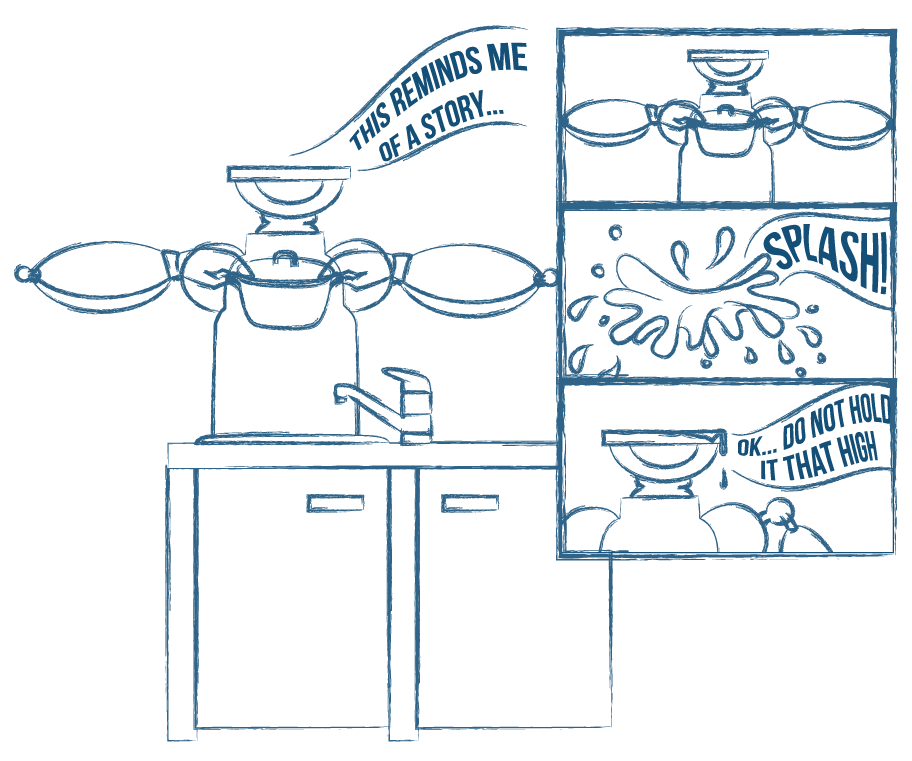
\includegraphics[width=12cm]{img/NarrativesStory.png}}
 \put(340,-10){
\includegraphics[width=4.0cm]{img/ease-logo.pdf}}}

\renewcommand\thesection{\thechapter.\arabic{section}}

% TODO: use current SOMA version?
\newcommand{\neemversion}{1.0~}
\newcommand{\neemexp}{NEEM-experience~}
\newcommand{\neemexps}{NEEM-experiences~}
\newcommand{\neemnar}{NEEM-narrative~}
\newcommand{\neembak}{NEEM-background~}
\newcommand{\neem}{NEEM~}
\newcommand{\neems}{NEEMs~}
\newcommand{\neemhub}{NEEM-hub~}
\newcommand{\tf}{tf~}
\newcommand{\openease}{openEASE~}
\newcommand{\ease}{EASE~}
\newcommand{\mongodb}{MongoDB~}
\newcommand{\cram}{CRAM~}
\newcommand{\knowrob}{KnowRob~}
\newcommand{\owl}{OWL~}
\newcommand{\pr}{PR2~}
\newcommand{\qudt}{Qudt~}
\newcommand{\boxy}{Boxy~}
\newcommand{\eg}{e.g.~}
\newcommand{\ros}{ROS~}
\newcommand{\soma}{SOMA~}
\newcommand{\dul}{DUL~}
\newcommand{\easeOwl}{EASE.owl~}
\newcommand{\easeAct}{EASE-ACT.owl~}
\newcommand{\easeObj}{EASE-OBJ.owl~}
\newcommand{\cramOwl}{cram\_failures.owl}
\newcommand{\cramentitytoreplace}[1]{\textless #1\textgreater}
\newcommand{\cramloggerpackage}{"cram-cloud-logger"~}
\newcommand{\owlClass}[1]{\textit{#1}}
\newcommand{\owlPredicate}[1]{\textit{#1}}
\newcommand{\f}{\mkern-2mu f\mkern-3mu}
\newcommand{\abox}{\mathcal{A}}
\newcommand{\tbox}{\mathcal{T}}
\newcommand{\concept}[1]{\emph{#1}}
\newcommand{\relation}[1]{\emph{#1}}

\makeatletter
\newcommand{\chapterauthor}[1]{%
  {\parindent0pt\vspace*{-25pt}%
  \linespread{1.1}\large\scshape#1%
  \par\nobreak\vspace*{35pt}}
  \@afterheading%
}
\makeatother

\renewcommand\tabularxcolumn[1]{m{#1}}
\newcolumntype{Y}{>{\centering\arraybackslash}X}
% % % % % % % % % % % % % % % % % % % % % % % %
% % % Prelude
% % % % % % % % % % % % % % % % % % % % % % % %
\newcommand{\givenODPNAME}{}
\newcommand{\givenODPINTENT}{}
\newcommand{\givenODPDEFINEDIN}{}
\newcommand{\givenODPGRAPHIC}{}
\newcommand{\givenODPEXAMPLES}{}
\newcommand{\givenODPQUESTION}{}
\newcommand{\ODPINTENT}[1]     {\renewcommand{\givenODPINTENT}{#1}}
\newcommand{\ODPDEFINEDIN}[1]  {\renewcommand{\givenODPDEFINEDIN}{#1}}
\newcommand{\ODPGRAPHIC}[1]    {\renewcommand{\givenODPGRAPHIC}{#1}}
\newcommand{\ODPEXAMPLES}[1]   {\renewcommand{\givenODPEXAMPLES}{#1}}
\newcommand{\ODPQUESTION}[1]   {\renewcommand{\givenODPQUESTION}{#1}}
\newcommand{\OPDinit}{
  \renewcommand{\givenODPINTENT}{REQUIRED!}
  \renewcommand{\givenODPDEFINEDIN}{REQUIRED!}
  \renewcommand{\givenODPGRAPHIC}{REQUIRED!}
  \renewcommand{\givenODPQUESTION}{}
  \renewcommand{\givenODPEXAMPLES}{}
  \renewcommand{\labelitemi}{$\mathbf{\sqsubseteq}$}
}

\newenvironment{ODP}[1]{
\OPDinit
\renewcommand{\givenODPNAME}{#1}
}{
%\givenODPDESCRIPTION
%\begin{figure}[htb!]
\vspace{0.2cm}
\begin{minipage}{0.55\textwidth}
\fcolorbox{easeblue!40}{easeblue!10}{\begin{tabular}{ p{1.8cm} p{4.2cm} }
%\toprule
% {\it\bf Name}                 & \emph{\givenODPNAME} \\
{\noindent\color{easeblue}\it\bf Intent}               & \givenODPINTENT \\
{\noindent\color{easeblue}\it\bf Competency Questions} & \emph{\givenODPQUESTION} \\
{\noindent\color{easeblue}\it\bf Defined in}           & \givenODPDEFINEDIN \\
%\bottomrule
\end{tabular}}
\end{minipage}
\begin{minipage}{0.45\textwidth}
\begin{center}
\givenODPGRAPHIC
\end{center}
\end{minipage}
\\[0.4cm]
\fcolorbox{easeblue!40}{easeblue!10}{
	\begin{minipage}{0.96\textwidth}
		\begin{tabular}{p{4.4cm}p{6.7cm}}
		{\noindent\color{easeblue}\it\bf Expression}  &
		{\noindent\color{easeblue}\it\bf Meaning} \\
		\givenODPEXAMPLES
		\end{tabular}
	\end{minipage}
}
%\caption{\emph{The Representation of \givenODPNAME}.}
%\end{figure}
\vspace{0.2cm}
}

\setcounter{tocdepth}{3}

\begin{document}
\let\oldaddcontentsline\addcontentsline
\def\addcontentsline#1#2#3{}
\maketitle
\def\addcontentsline#1#2#3{\oldaddcontentsline{#1}{#2}{#3}}

\begin{abstract}
The Collaborative Research Center \ease is an interdisciplinary research initiative at the University of Bremen that attempts to advance our understanding of how human-scale manipulation tasks can be mastered by robotic agents.
The challenge is that the same task needs to be executed by the robot in different ways depending on, for example, what tools are available, and how the environment is shaped.
The key to solve this issue is \emph{generalization}.
However, the robot needs to know more then what step it needs to execute next -- it further needs to decide on how the next step is carried out through motions of its body, and interactions with its environment.
In this document, we will describe how these types of information are represented in the \ease system, how such data-sets are acquired, and how they are stored, maintained, and curated using a centralized web-service.
The goal of this effort is to establish representations and infrastructure for a shared experience storage with annotated data-sets of agents performing everyday activities,
and to use these data-sets as ground truth data to find generalizations that do not abstract away from movements, and naive physics.
\end{abstract}

\cleardoublepage
\tableofcontents

\pagenumbering{arabic}
\setcounter{page}{0}
\cleardoublepage
\chapter{Introduction}
\chapterauthor{D. Be{\ss}ler, S. Koralewski, M. Pomarlan}

This document, referred to as the ``\neem Handbook'' hereafter,
describes the \ease system for episodic memories of everyday activities.
%The \neem Handbook will be updated along the progress in the CRC \ease.
It is thought to provide \ease researchers with compact but still comprehensive
information about what information is contained in \neems,
how it is represented, acquired, curated and published.

\begin{figure}[h!]
\centering
\begin{tikzpicture}[
    border/.style={draw=easeblue},
    dark/.style={border,fill=easeblue!20},
    light/.style={border,fill=easeblue!10},
    lighter/.style={border,fill=easeblue!5},
    heading/.style={text=easeblue,font=\bf,text badly centered},
    label1/.style={text=easeblue,text badly centered},
    label2/.style={text=black,text badly centered,font=\it},
    label/.style={text=black,text width=1.7cm,text badly centered},
    hexagon/.style={regular polygon,regular polygon sides=6,rounded corners},
    triangle/.style={regular polygon,regular polygon sides=3,rounded corners},
    trapez/.style={font=\bf,text badly centered,trapezium,trapezium angle=60,rounded corners},
    user/.style={hexagon,lighter,minimum width=2.5cm,inner sep=0},
    img/.style={}
]
  %\draw[help lines](-4,-4)grid(4,3);
  %% outer hexagon
  \node[hexagon,dark,minimum width=5.0cm] (OUTER) {};
  \node[heading] at (0,-1.8) (ACQ) {acquisition};
  \node[heading,rotate around={120:(OUTER)},rotate=180] at (ACQ) {curation};
  \node[heading,rotate around={-120:(OUTER)},rotate=180] at (ACQ) {publication};
  %% inner triangle
  \node[triangle,light,minimum width=6.0cm] at (OUTER) (INNER) {};
  %% inner trapez
  \node[trapez,lighter,
    minimum height=21mm,yshift=-0.275cm] at (INNER.center) (LIB) {};
  \node[label,yshift=0.2cm] at (INNER) (BG) {NEEM Background};
  \node[label,below=0.2cm of BG.south,anchor=north east] (NAR) {NEEM Narrative};
  \node[label,below=0.2cm of BG.south,anchor=north west] (EXP) {NEEM Experience};
  \draw[draw=easeblue] (BG.south west) -- (BG.south east);
  \draw[draw=easeblue] (NAR.north east) -- (NAR.south east);
  %% heading
  \node[label1,text width=14mm,above=0.4cm of BG] (HUB1) {NEEM HUB};
  %%
  \node[user,text=black,anchor=north,yshift=-0.2cm,
    path picture={\node[yshift=1.8cm] at (path picture bounding box.center){
        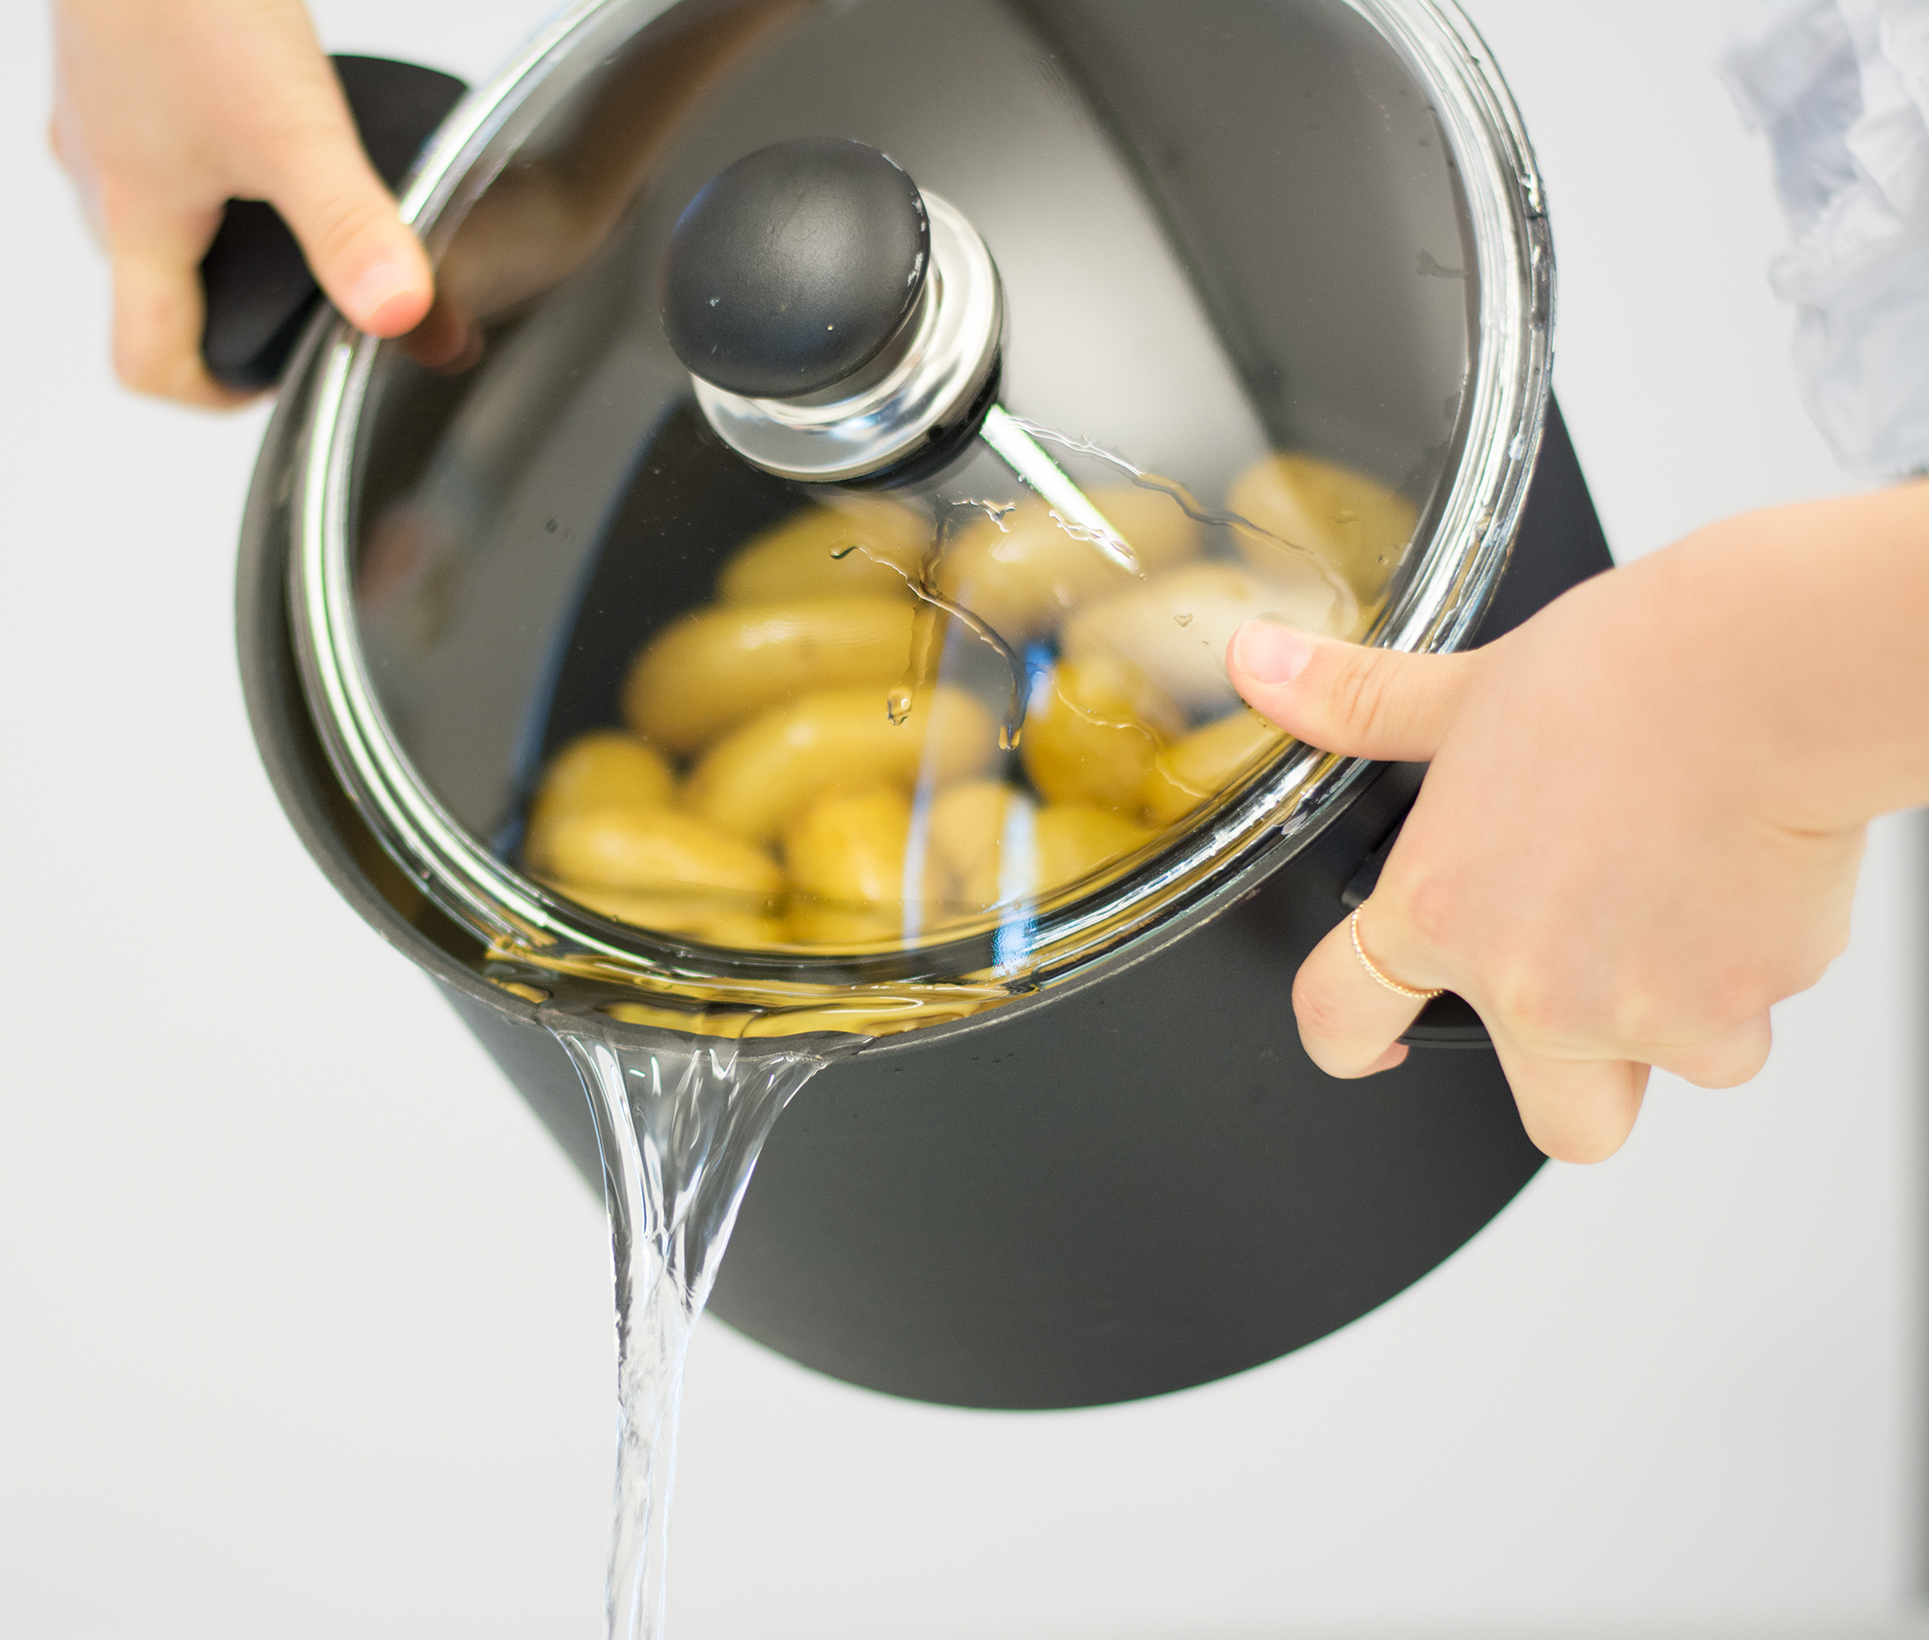
\includegraphics[width=2.55cm]{img/topf-2.jpg}
    };}
  ] at (OUTER.south) (X1) {};
  \node[user,anchor=center,yshift=-0.4cm,xshift=2.4cm,
    path picture={\node[yshift=0.0cm] at (path picture bounding box.center){
        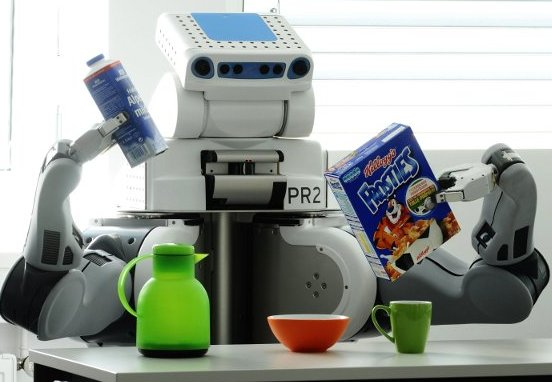
\includegraphics[height=2.55cm]{img/pr2_milk_frosties_small_top.jpg}
    };}
  ] at (X1.north) (X2) {};
  \node[user,anchor=center,yshift=-0.4cm,xshift=-2.4cm,
    path picture={\node[yshift=0.0cm] at (path picture bounding box.center){
        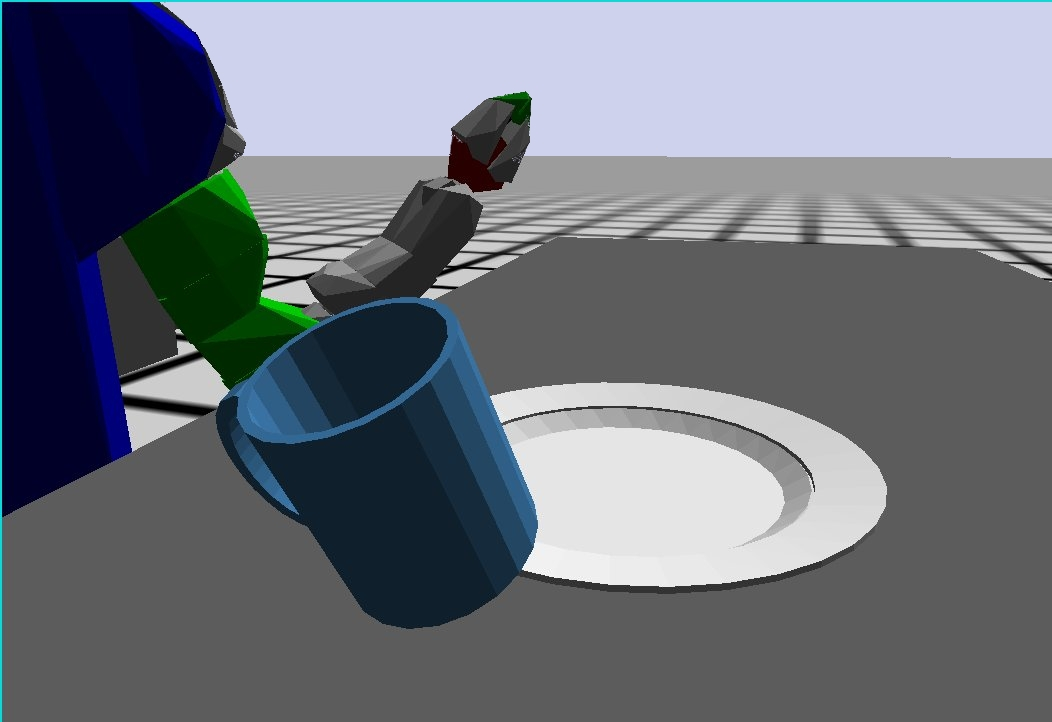
\includegraphics[height=2.55cm]{img/cup-on-plate-unstable-final.jpg}
    };}
  ] at (X1.north) (X5) {};
  \node[user,rotate around={120:(OUTER)},
    path picture={\node[yshift=0.0cm] at (path picture bounding box.center){
        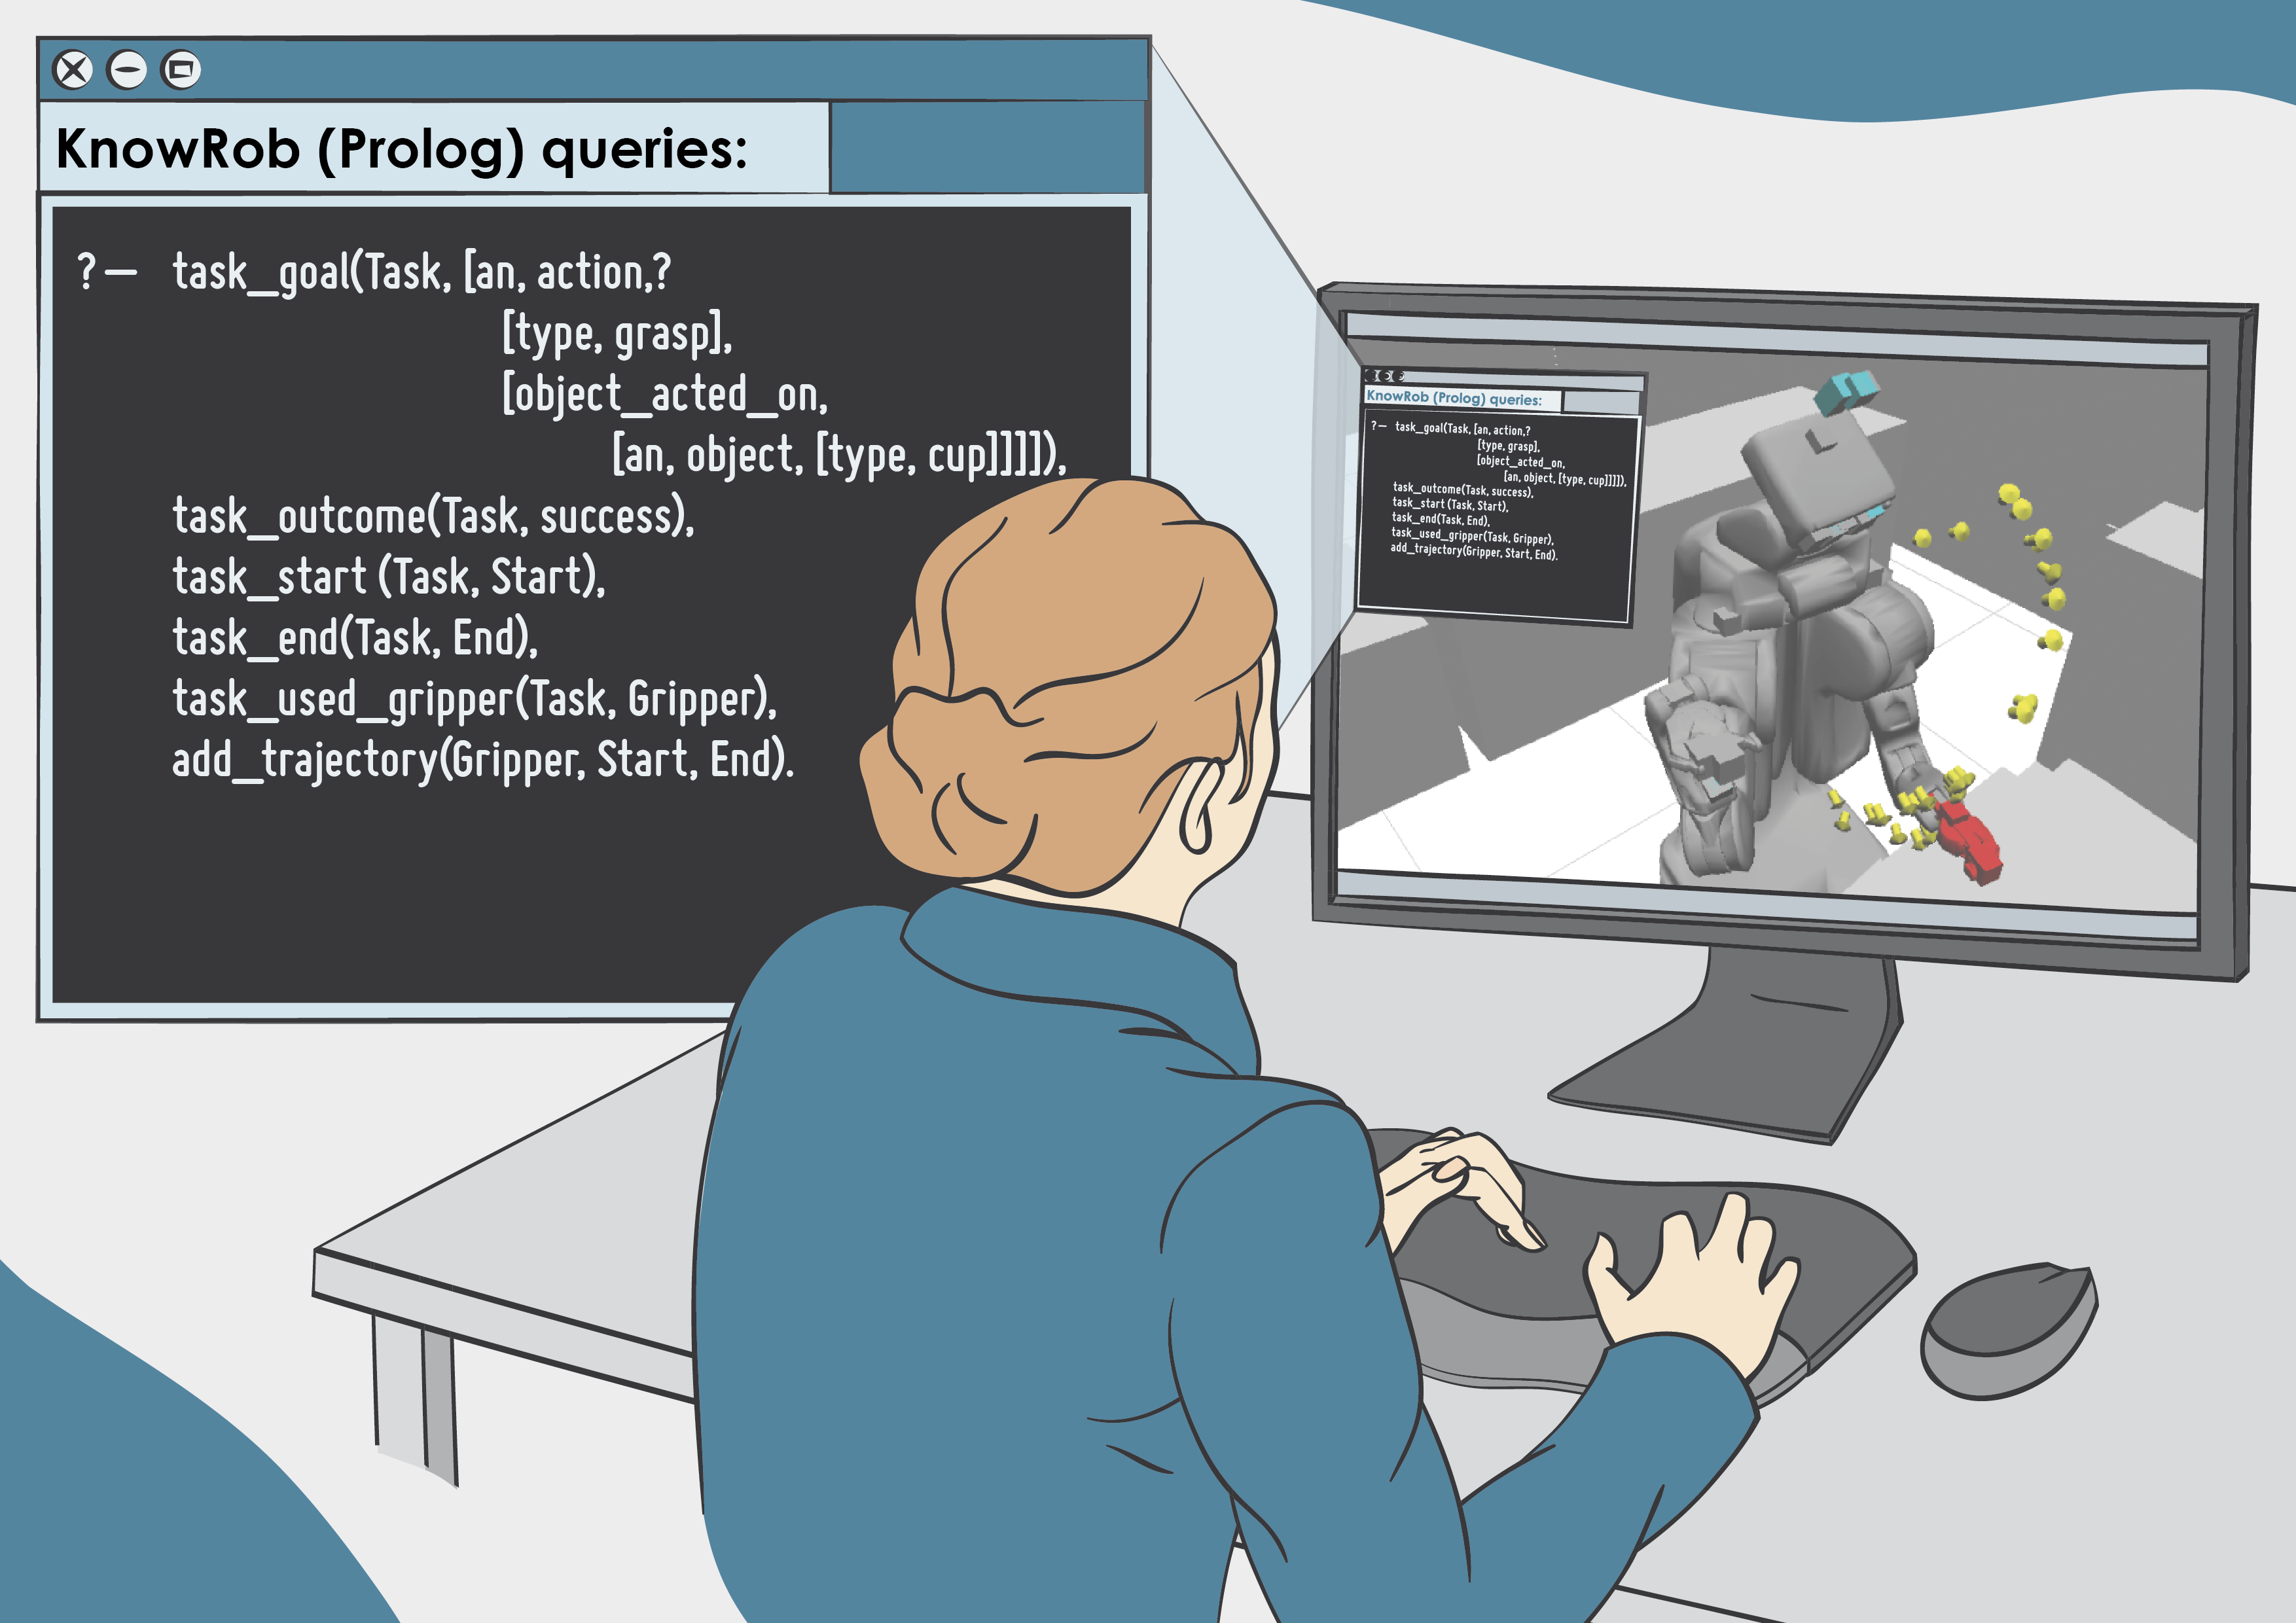
\includegraphics[height=2.55cm]{img/Programmer.png}
    };}
  ] at (X1) (X3) {};
  \node[user,rotate around={-120:(OUTER)},
    path picture={\node[yshift=0.0cm] at (path picture bounding box.center){
        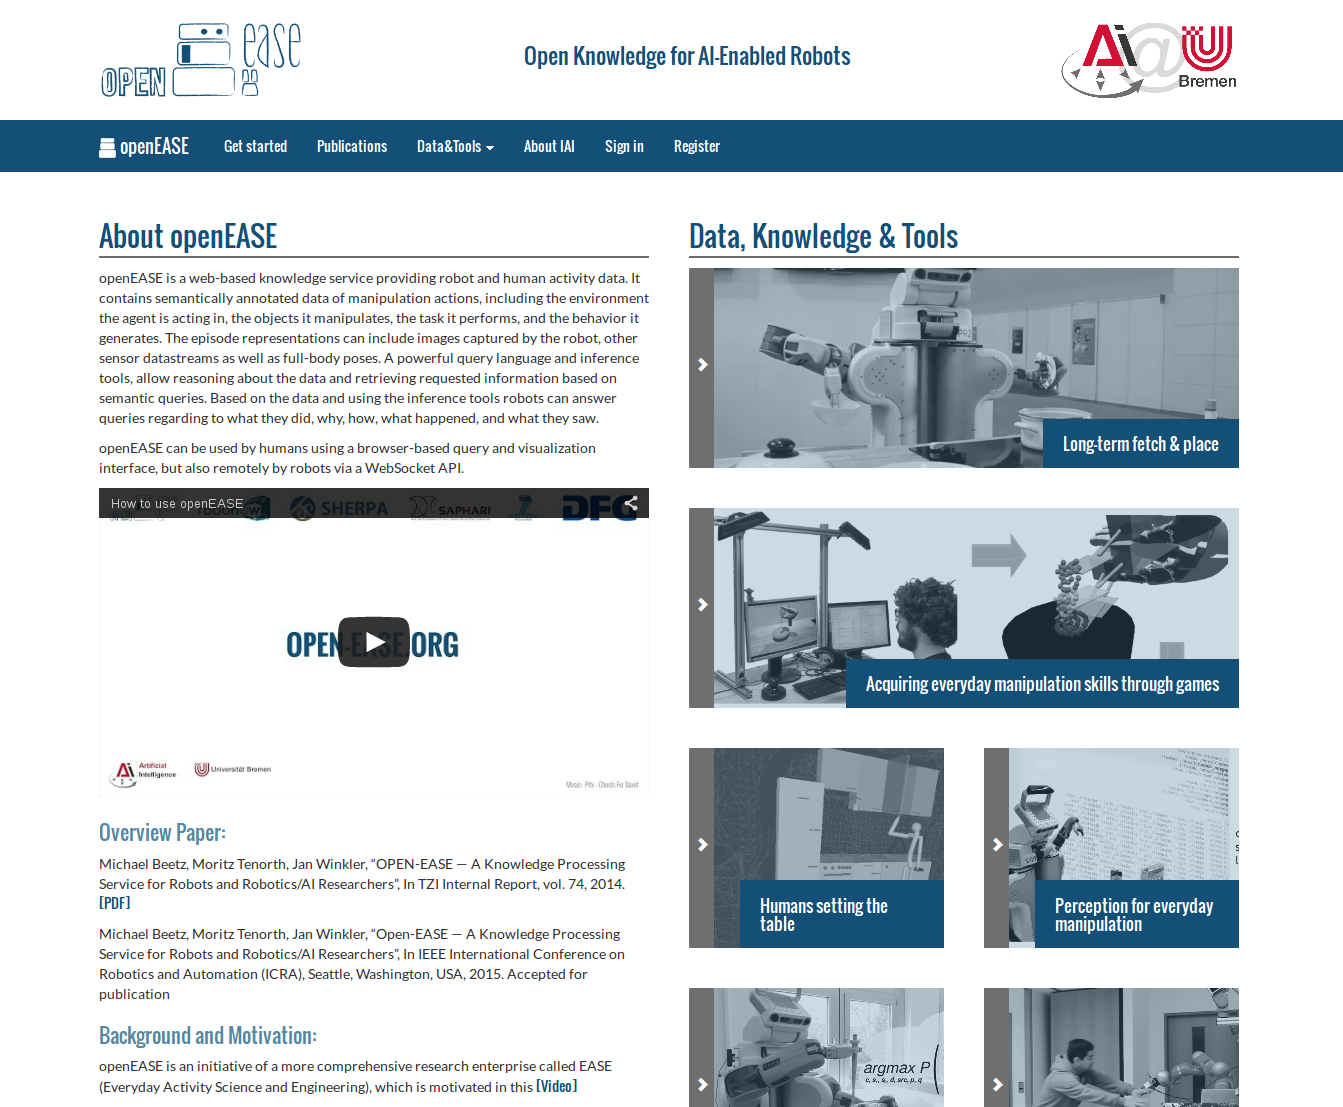
\includegraphics[height=2.55cm]{img/open-ease-web-page-full_cropped.png}
    };}
  ] at (X1) (X4) {};
  %%
  \node[label2,anchor=north] at (X1.south) {observation};
  \node[label2,anchor=north] at (X2.south) {experimentation};
  \node[label2,anchor=north] at (X5.south) {simulation};
  
\end{tikzpicture}
\caption{The EASE system for acquisition, curation and publication of episodic memories}
\label{fig:architecture}
\end{figure}

\paragraph{Narrative Enabled Episodic Memories}
% From KnowRob 2.0
When somebody talks about the deciding goal in the last soccer world championship many of us can ``replay'' the episode in our ``mind's eye''.
Those episodic memories can be seen as abstract descriptions that allow us to recall detailed pieces of information from any experienced activity.
Having those detailed memories, we can use them to learn general knowledge or map similar memories to unknown situations, so we know how to behave in the given situation.
\todo{DB: refer to Figure~\ref{fig:architecture}}

% From KnowRob 2.0
\ease integrates episodic memories deeply into the knowledge acquisition, representation, and processing system. 
For every activity the agent performs, observes, prospects and reads about, it creates an episode and stores it in its memory.
An episode is best understood as a video recording that the agent makes of the ongoing activity.
In addition, those videos are enriched with a very detailed story about the actions, motions, their purposes, effects and the agent's sensor information during the activity.

% From KnowRob 2.0
We define the episodic memories created by our system narrative-enabled episodic memories (\neems).
A \neem consists of the \emph{\neem experience} and the \emph{\neem narrative}.
The \neem experience captures low-level data such as the agent's sensor information, e.g. images and forces, and records of poses of the agent and its detected objects.
\neem experiences are linked to \neem narratives, which are stories of the episode described symbolically.
These narratives contain information regarding the tasks, the context, intended goals, observed effects, etc.
The \neemexp and \neemnar combined are so rich of information that the agent can replay an episode to experience the seen activity anytime again.

\neems are representations of experiences acquired through experimentation, reading, observing, mental simulation, etc.
The main goal is to establish a common vocabulary used to annotate experience data across different tasks, scientific disciplines, and modalities of acquisition, and to define models for the representation of experience data.
The vocabulary is not just a set of atomic labels, but each label has a formal definition in an ontology.
These definitions are done such that a set of \emph{competency questions} about an activitiy can be answered by a knowledge base that is equipped with the ontology and a collection of \neems.

The \neem model is formally defined in form of an \owl ontology which is based on the DOLCE+DnS Ultralite (DUL) upper-level ontology~\cite{DOLCE2003}.
DUL is a carefully designed ontology that seeks to model general categories underlying human cognition without making any discipline-specific assumptions.
Our extensions of DUL mainly focus on characterizing different aspects of activities that were not considered in much detail in DUL, but are relevant for the autonomous robotics scope.
These extensions are part of an ontology that we have called
\soma~\footnote{\url{https://ease-crc.github.io/soma}}.
A \neem is made of several patterns defined either in \dul or in \soma.

While it is possible to create the representations listed in this document through a custom exporter, it is not advised to do so.
Instead, it is advised to interface with the
\knowrob knowledge base~\footnote{\url{https://github.com/knowrob/knowrob}}.
\knowrob provides an interface based on predicate logics that allows to interact with \neems.
The language is a collection of predicates that can be called by users to ask certain types of competency questions covering different aspects of activitiy, or to add labels and relationships in the \neemnar.
We will provide example expressions in this document that highlight how the knowledge base can be used to interact with \neems.

% paragraph about generalizability of robot behaviour (add reference to Pratt paper ``Is a Cambrian Explosion Coming for Robotics?'')
%\lipsum[4]
%\todo{DB: write paragraph about generalizability, Pratt paper ``Is a Cambrian Explosion Coming for Robotics?''}

% % % % % % % % % % % % % % % % %
% % % % % % % % % % % % % % % % %
\section{Notation} % Domain of Discourse
\label{sec:notation}

In this Section, we will shortly introduce the notions and notations that are important to follow this document.
%Because in subsequent sections we will give more formal definitions for various concepts, we now review some basic notions about the main formalism we use in the ontology, as well as introduce the notation we will employ.

%%% ABOX -- TBOX
\neems are formally represented using an \emph{ontology}.
An ontology is a collection of logical axioms in some formal language such as description logic (DL).
%In the case of many ontologies available in the semantic web, as well as in the case of SOMA, this formal language is description logic, also known as DL.
The entities that can be described in DL can be either \emph{concepts} (sometimes known as \emph{classes}),
and \todo{Seba: Can we here remove individuals? It seems not very well definied that concepts are known as individuals and in the next sentence the instances are called individuals. MP: I checked the Description Logic Primer, and they use individuals. I think we should keep this.}
\emph{instances}.
An individual may belong to one or more concepts.
A concept may be subsumed by another concept.
Between individuals there may be relations called \emph{object properties},
and, in addition, an individual can also have \emph{data properties} that link it to some data values.
%As a syntactic convenience, an individual can also have ``data properties'' that link it to some alphanumeric data item which is itself not considered an individual in the ontology.
As an example, let us assume that Alice and Bob are both individuals belonging to the concept \concept{Human},
and that the object property \relation{hasChild} connects Alice to Bob,
i.e. the relation asserts that Bob is a child of Alice.
We may also know the height of Alice, which would be represented by a data property \relation{hasHeight} whose value could be a string such as \emph{1,7m} to represent that she is 1.7m tall.
%%
In the following, to make clear when we are talking about concepts and when about individuals, we will denote the set of all concepts as $\mathcal{T}$ (called the TBox), and the set of all individuals as $\mathcal{A}$ (called the ABox).
%Accordingly, there are axioms that describe concepts or object/data properties,
%and axioms that describe individuals and the relations between them.
%The set of concepts, object and data properties, and the axioms that
%define them is called the Tbox, or terminological part,
%and we will denote it by $\mathcal{T}$.
%The set of individuals and the axioms describing them is called the Abox,
%or assertion part, and we will denote it by $\mathcal{A}$.

%%% formatting
It is useful when describing concepts to emphasize the concept names such that it is clear we reference the concept, and not the colloquial word. As such, \concept{Concepts} and \relation{relations} will be written in a different font.
Note that the name of a concept always starts with an uppercase letter, whereas the name of a relation with a lowercase one.
Any word appearing in a concept or relation name after the first one will always begin with an uppercase letter.

%%% namespaces
Ontologies are meant to build on one another, and it is not uncommon for an ontology to collect thousands of concepts from external ontologies it imports.
To prevent name clashes, in actual usage the names of concepts, relations, and individuals are often name-spaced.
In this document, since we mostly talk about concepts from the SOMA ontologies,
the namespace will not be made explicit.
An exception will be made in some diagrams where we reference concepts defined in more basic ontologies,
such as those used to define the Ontology Web Language (OWL).
An example is a name such as \emph{xsd:double}; in this case, \emph{xsd} is the namespace.

% % % % % % % % % % % % % % % % %
% % % % % % % % % % % % % % % % %
\section{Scope} % Domain of Discourse
\label{sec:scope}

The broad scope of this work is to provide information about how robotic manipulation activities are represented, acquired, curated and published in the \ease system for episodic memories.
%Our work aims to provide knowledge modeling for robotic manipulation and autonomous robot control, such that data acquired through performing actions can be stored, interpreted, and used towards training and improving robot skills.
%The knowledge that is to be extracted from data must include 
We are in particular interested in
aspects of interaction forces and motion characteristics of objects participating in an action, since it is these physical and geometric considerations that are crucial for successfull action execution.
%determine whether, or to what degree, an action is successful.
The goal is to learn models from collections of recorded data semantically annotated through concepts defined in the \neem model.
The rich semantic annotations enable querying and filtering the data, such that a robot can formalize a learning problem for itself and curate its training data to be appropriate for it.
Information about how the data is collected, with what methods, from what agents, in which contexts, is important for this process, as machine learning techniques are sensitive to training data biases.
Note that in principle episodes can be stored of any agent performing any activity, and in actuality many of the NEEMs we expect to store will come from humans demonstrating how to perform a task.
NEEMs are therefore not simply intended as a kind of self-practice journal, but rather as a store of practical knowledge of a variety of agents, useful for a variety of autonomous, humanoid robots.

The kinds of knowledge a robot needs for competent performance of its tasks are varied. Usually, knowledge modelling in robotics and AI has focused on a symbolic level, of actions treated as black boxes that relate to a larger plan by means of their preconditions and effects. Actions are also very underspecified when described in spoken commands. This abstract level of description however is insufficient; the physical details of the actions matter. For example, the angle and speed with which a pitcher is moved, and the amount of liquid in it, determines whether there will be spillage. A robot needs to choose appropriate parameters for its actions, and infer these parameters when they are left unspecified in a command.

Such inference requires the robotic agent to be equipped with common-sense and intuitive physics knowledge, as well as an abstract task and object model, and knowledge of how to apply these models in a given situation.
The \neem model attempts to support each of these requirements.
A brief list of some of the over-arching competency questions follows.

\begin{itemize}
    \item \emph{How are actions conceptualized?} What is an action, how does it relate to other concepts an agent might have about the world? What is the purpose of an action?
    \item \emph{What is the structure of an action?} How do several actions make up another? What objects participate in an action and with what roles?
    \item \emph{How are qualitative and quantitative features of the world represented?} What is the parameter set of an action? What regions can values for these parameters occupy? What is a good parameterization and how can one be found?
    \item \emph{How are the physical interactions that underlie an action described?} What are the involved forces, and how are they parameterized? What are relevant qualitative, and thus more general, descriptors for interactions, such as balance, blockage, compulsion? How are qualitative aspects of interaction grounded in quantitative physical phenomena?
    \item \emph{How are objects conceptualized?} What roles can an object play? What actions can it take part in? What kinds of objects are necessary for an action?
    \item \emph{How is an action recorded and described?} What is the relevant data to capture how an action unfolded? What are the relevant pieces of contextual information for describing an action that has actually occurred? What was the outcome of the action, in particular, to what extent did it match the goal?
    \item \emph{How is a learning problem formalized?} What is the optimization goal? What assumptions were in effect when collecting the training data? What sort of influence might biases have upon the learned model? What should be essential features that a learned model should use? What would be sanity checks on the learned model to verify it does not abuse spurious correlations?
\end{itemize}

% % % % % % % % % % % % % % % % %
% % % % % % % % % % % % % % % % %
\section{Overview}
\label{sec:overview}

% paragraph about the intention behind this document
\neems are the central data structures that link research results of various sub-areas within the collaborative research center \ease.
\ease is an interdisciplinary institution headed by leading researchers in the fields robotics, human cognition, formal logics, and linguistics.
The overall goal is to make a robot more competent in performing everyday activities.
This is accomplished by equipping the robot with models learned over experiences represented as \neems.
The purpose of this document is to provide detailed information about the \ease system for episodic memories.
That is how \neems are
represented as knowledge bases linked to time-series data,
acquired through experimentation, observation or simulation,
stored on a centralized server, and
maintained as a dataset for the research community.
The architecture is shown in Figure~\ref{fig:architecture}, and will be summarized in the remainder of this section.

% paragraph about representation (neem background, narrative, experience)
At the core of the \ease system for episodic memories is the \neem data structure.
It is a heterogenous datastructure that contains data in different formats to represent different categories of information about everyday activities.
Each \neem is made of three parts: background (Chapter~\ref{ch:background}), narrative (Chapter~\ref{ch:narrative}) and experience (Chapter~\ref{ch:experience}).
The background represents physical activity context by characterizing the environment, and agents that play a role during the activity.
A single background may be shared in mutiple \neems.
The narrative is a representation of events that happened, their characterization and contextualization.
That is, for example, that an event occurred, what roles objects played during the event, how the event was carried out through motions and interactions, and what the reason of its occurrence is.
The narrative provides labels used to annotate the time-series data stored in the experience of the \neem.
This is done by associating the event time intervals to slices in the time-series database.
The experience data is used to capture some aspects of kinematics and dynamics of an activity, that is how objects moved, how they got into contact with each other, and how forces act upon objects.

% paragraph about neem hub -- purpose, potential, ... -- add some buzzwords from data science
\neems are stored on a publicly accessible infrastructure that we have called the \neemhub (Chapter~\ref{ch:neemhub}).
The \neemhub builds on top of common infrastructure used in data science to continuously update models learned from \neems.
Uploading a \neem requires to create a new data set on the \neemhub GitLab interface where users can provide documentation, usage examples, additional links and references for their \neem data set.
Once a user is satisfied with the state of the data set, it may be published.
This will make the data set accessible via the knowledge service \openease where users may search for data sets given some keywords, download the data set, or investigate it in an interactive environment.

% paragraph about acquisition (robot, vr) -- what do they have in common? what is different?
As \ease is an interdisciplinary effort, there are also different modalities under which \neems can be acquired.
We haved developed multiple acquisition infrastructures that support researchers from different domains to acquire \neems (Chapter~\ref{ch:acquisition}).
This is, first of all, an interface that integrates with a robot control system either in a simulated or real-world scenario where the robot senses its surroundings, and executes specific plans through motions of its body and interactions with its environment.
A second acquisition interface integrates with simulated virtual reality environments in which humans perform everyday activities.
In this case, the intentions are not certainly known because even when told to do something specific, a human may do some unrelated experimentation in the virtual reality.
The state of the environment including force characteristics can, however, fully be monitored.


%\input{content/requirements/requirements}
%\input{content/representation/representation}

\setcounter{section}{0}
\input{content/representation/neem-background}

\setcounter{section}{0}
\input{content/representation/neem-narrative/neem-narrative}

\setcounter{section}{0}
\chapter{NEEM-Experience}
\label{ch:experience}
\chapterauthor{D. Be{\ss}ler, S. Koralewski}

\neemexp captures low-level information about experienced activities
represented as time series data streams.
This data has often no or only unfeasible
lossless representation as facts in a knowledge base.
To make this data \emph{knowledgable}, procedural hooks
are defined in the ontology to compute symbols from the experience data,
and to embed these symbols in logic-based reasoning.

The data is stored in a NoSQL database using JSON documents.
Each individual type of data is stored in a separate collection
named according to the type of data stored in the collection.
When imported, the knowledge system stores the data in a
\mongodb\footnote{https://www.mongodb.com/} server, for which
the knowledge system implements a client for querying the data
during question answering.
The query cursor concept employed in \mongodb integrates
nicely with backtracking based search employed in the knowledge system.
It further scales well to large amount of data and can be distributed amongst
clusters through built-in automatic sharding.

The data in \neemexps is represented as time series
and indexed in time order.
The different experience data types need to define a dedicated
time key for computing the search index.

% the \neemexp consists only of \tf data \cite{tf}.
% When executing an experiment in projection, we are collecting \tf data from the map, objects and the robot.
% In real world experiments we log only the \tf data from the map and the robotic agent.
% We are storing the \tf data in a \mongodb\footnote{https://www.mongodb.com/}.
% In the next iteration of the document we will provide links where you can download the required tools for log \tf data for NEEMs.

The experience data in \neems has individual characteristics regarding
the format, compressed representation, and what symbols the 
knowledge system can abstract from the data.
In this chapter, we describe these aspects for the experience data types covered 
in \neem version \neemversion.

%%%%%%%%%%%%%%%%%%%%%%%%%%%%%%%%%
%%%%%%%%%%%%%%%%%%%%%%%%%%%%%%%%%
\section{Kinematics}

%%%%%%%%%%%%%%%%%%%%%%%%%%%%%%%%%
\subsection{Pose data}

A robotic system typically has many mobile components arranged in a kinematic chain.
Each component in a kinematic chain has an associated named coordinate frame such as
world frame, base frame, gripper frame, head frame, etc.
Coordinate systems are always 3D, with \emph{x} forward, \emph{y} left, and \emph{z} up, which follows the \textbf{right handed} coordinate system.
6 DOF relative poses are assigned to the different frames.
These are usually updated with about 10 Hz during movements, and
expressed relative to the 
parent in the kinematic chain to avoid updates when only the parent frame moves.
The transformation tree is rooted in the dedicated world frame node
(also often called map frame).

The data is used by the \ease knowledge system to answer questions such as:
\begin{itemize}
% questions taken from TF docu page
 \item Where was the head frame relative to the world frame, 5 seconds ago?
 \item What is the pose of the object in the gripper relative to the base?
 \item What is the pose of the base frame in the map frame? 
\end{itemize}

% \begin{center}
% 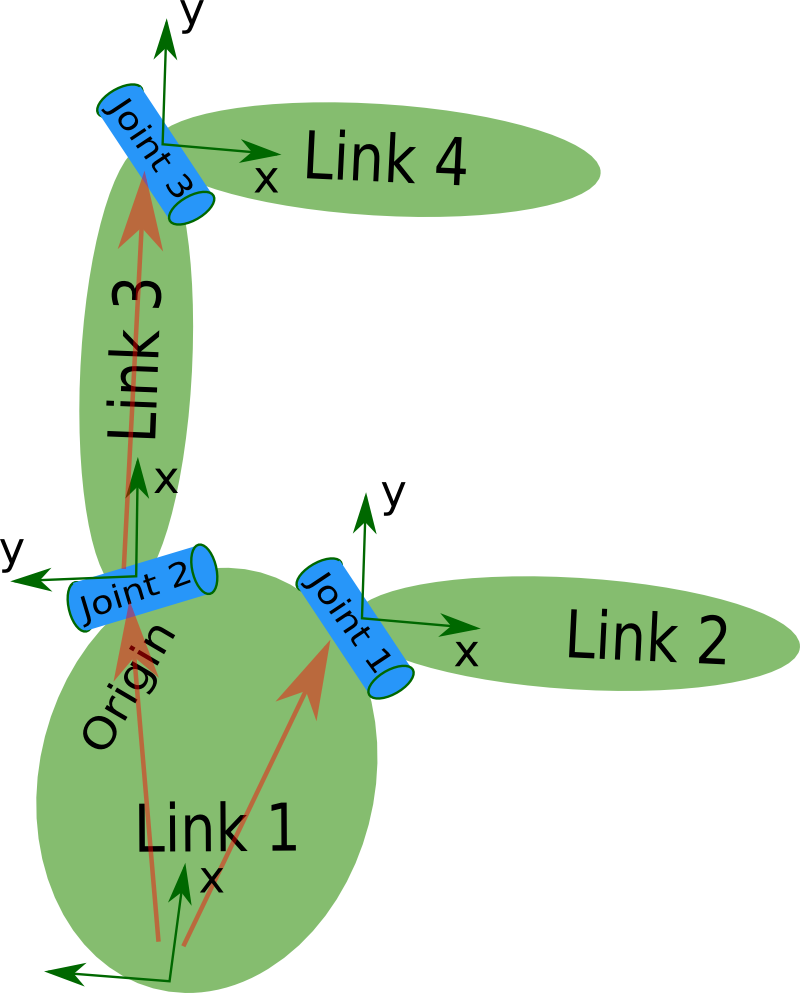
\includegraphics[height=0.3\textwidth]{img/links-joints.png}
% 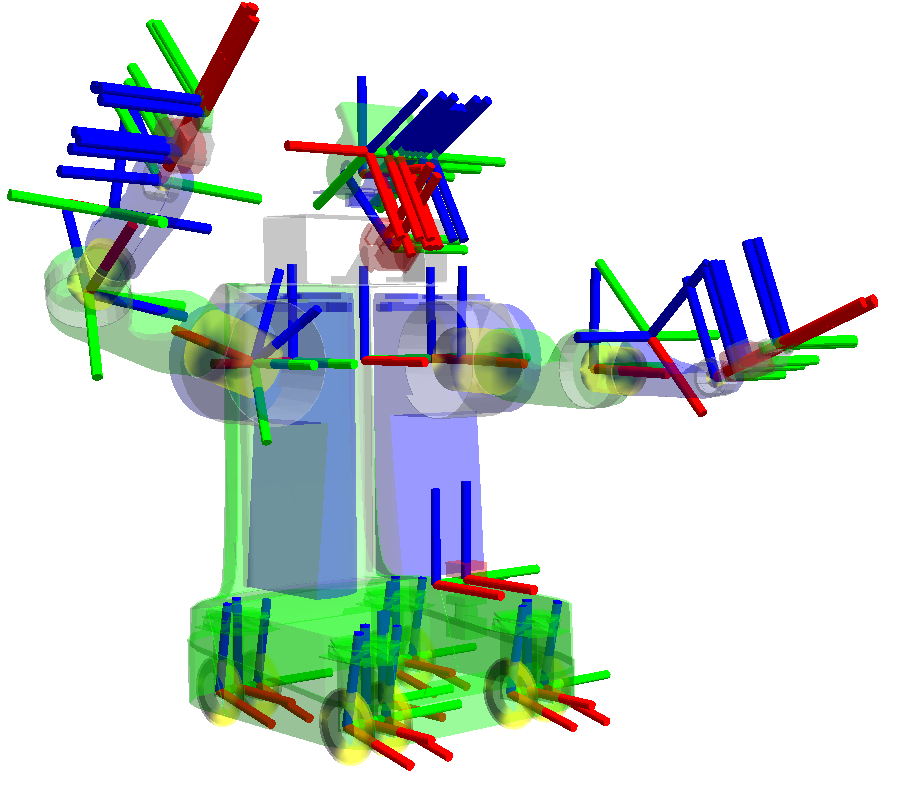
\includegraphics[height=0.3\textwidth]{img/tf-frames.png}
% \end{center}

Pose data is saved in \mongodb collections named ``tf'', the format is described below.

%%%%%%%%%%%%%%%%%%%%%%%%%%%%%%%%%
%%%%%%%%%%%%%%%%%%%%%%%%%%%%%%%%%
\paragraph{Format}
The pose data structure has
fields for encoding the translation and rotation of a coordinate frame.
The parent frame and time stamp of pose estimation
are stored in the \emph{header} field of the data structure.
The transform coordinate frame is assigned to the \emph{child\_frame\_id} field. \\

%The data is stored in the DB collection as array. Each array holding pose estimates for distinct frames at the same time stamp. For indexed search, it is important that each array member has the same time stamp. \\

\def\arraystretch{1.1}%
\begin{figure}[htb]
\begin{center}\begin{tabular}{ >{\ttfamily}p{3.5cm} >{\ttfamily}p{2cm} p{5cm} }
\toprule
\bf Field   & \bf Type & \bf Description \\ \midrule
tf			& dict	& -- \\
\ \ header		& dict		& -- \\
\ \ \ \ seq		& uint32	& consecutively increasing ID \\
\ \ \ \ stamp		& time		& time stamp of this transform \\
\ \ \ \ frame\_id	& string	& parent coordinate frame of this transform \\
\ \ child\_frame\_id	& string	& coordinate frame of this transform \\
\ \ transform		& dict		& -- \\
\ \ \ \ translation	& dict		& position of child frame with respect to parent frame in meters \\
\ \ \ \ \ \ x		& float64	& \emph{x} axis translation \\
\ \ \ \ \ \ y		& float64	& \emph{y} axis translation \\
\ \ \ \ \ \ z		& float64	& \emph{z} axis translation \\
\ \ \ \ rotation	& dict		& -- \\
\ \ \ \ \ \ x		& float64	& \emph{x} component of quaternion \\
\ \ \ \ \ \ y		& float64	& \emph{y} component of quaternion \\
\ \ \ \ \ \ z		& float64	& \emph{z} component of quaternion \\
\ \ \ \ \ \ w		& float64	& \emph{w} component of quaternion \\
\bottomrule
\end{tabular}\end{center}
\caption{The pose data structure in the \ease system.}
\label{fig:pose_data}
\end{figure}

Note that static frames may be recorded at lower frequency --
about every two seconds.
This usually reduces the data size significantly.
At the moment, no other motion data compression,
such as motion JPEG, is supported.

% From ``Compression of Motion Capture Databases'' Okan Arikan
% The biggest goal of compression is creating a compressed rep-
% resentation of motion that is perceptually as close to the original
% motion as possible. As we will explore later in this paper, a small
% numerical error does not necessarily correspond to a perceptually
% close motion. We would like compression and decompression to be
% as quick as possible. In practice motion capture databases can be
% very big. Therefore another goal for compression and decompres-
% sion is to be able to process without holding the entire database in
% the memory, which may not be possible. Depending on the appli-
% cation we may want to “stream” the data so that the decompressor
% can decode incrementally. We may also want to be able to decode a
% piece of the database without having to decompress any other mo-
% tion



%%%%%%%%%%%%%%%%%%%%%%%%%%%%%%%%%
%\subsection{Joint state}
%\lipsum[2] \todo{explain how joint state is stored in neem experience}

%%%%%%%%%%%%%%%%%%%%%%%%%%%%%%%%%
%%%%%%%%%%%%%%%%%%%%%%%%%%%%%%%%%
%\section{Dynamics}

%%%%%%%%%%%%%%%%%%%%%%%%%%%%%%%%%
%\subsection{Net force}

%\lipsum[2] \todo{explain how net force is stored in neem experience}

%%%%%%%%%%%%%%%%%%%%%%%%%%%%%%%%%
%%%%%%%%%%%%%%%%%%%%%%%%%%%%%%%%%
% \section{Image Data}
% \input{content/neem-experience/image-data}

%%%%%%%%%%%%%%%%%%%%%%%%%%%%%%%%%
%%%%%%%%%%%%%%%%%%%%%%%%%%%%%%%%%
% \section{Gaze Data}
% \input{content/neem-experience/gaze-data}

%%%%%%%%%%%%%%%%%%%%%%%%%%%%%%%%%
%%%%%%%%%%%%%%%%%%%%%%%%%%%%%%%%%
% \section{EEG Data}
% \input{content/neem-experience/eeg-data}


\setcounter{section}{0}
\chapter{NEEM-Hub}
\label{ch:neemhub}
\lstset{style=lispcode}
\chapterauthor{S. Koralewski, S. Jongebloed}


Our CRC aims to acquire a huge amount of data, make the data accessible to the research community,  allow to analyze the data, create machine learning models from the data and support version control for the data and models. 
With our \neemhub concept we are covering all those requirements with one system.

To implement the version control of large data sets and machine learning models, we are using DVC\footnote{\url{https://dvc.org/}}. 
We use Hadoop\footnote{\url{https://hadoop.apache.org/}} and its file system HDFS to store the data and models.
Hadoop is a cluster system which creates automatically replicas of the data once it is uploaded and allows parallel processing of data to speed up transforming or querying the data.

On a high level perspective we want to realize two pipelines with our \neemhub as depict in Figure \ref{fig:neem-hub}.
The first pipeline can be seen as the acquisition and analytic pipeline.
The first step in the pipline is storing raw data, such as videos, text, images and electrocardiogram (ECG) data.
In the next step, so called neemifier are transforming this raw data into \neems which are utilizing the semantically representation provided by \soma.
Since we are using Hadoop, multiple instances of the same neemifier can neemify the raw data in parallel. 
There is also the possibility to upload \neems directly to the \neemhub, so the neemifing step can be skipped.
The stored \neems can be accessed by \openease. 
\openease allows the inspection and visualization of each individual \neem.
A direct download of the \neems to a local system is also supported.

The second pipeline should be used as a pipeline for learning from the acquired data.
\neems are so rich full on information that one \neem can be used for multiple learning problems.
In addition, \neems allow to generate models with different levels of abstraction. 
One can learn general models e.g.\ the likely location of perishable items or/and specialized models e.g. how an agent should grasp my favorite mug in my kitchen.
The procedure to generate the models is that transformers are used to extract the required features from the \neems and store them in a data representation, e.g.\ CSV, required for the machine learning model.
The learners, which create the models, store the data in the model library. 
This model library can be used afterwards by an agent to perform reasoning.

In some scenarios those two pipelines can be combined to create a closed-loop. 
A possible scenario can be a robot acquiring \neems, uploading them to the \neemhub and download afterwards the new models to improve itself for the next experiment. 


\begin{figure}[h!]
	\centering
	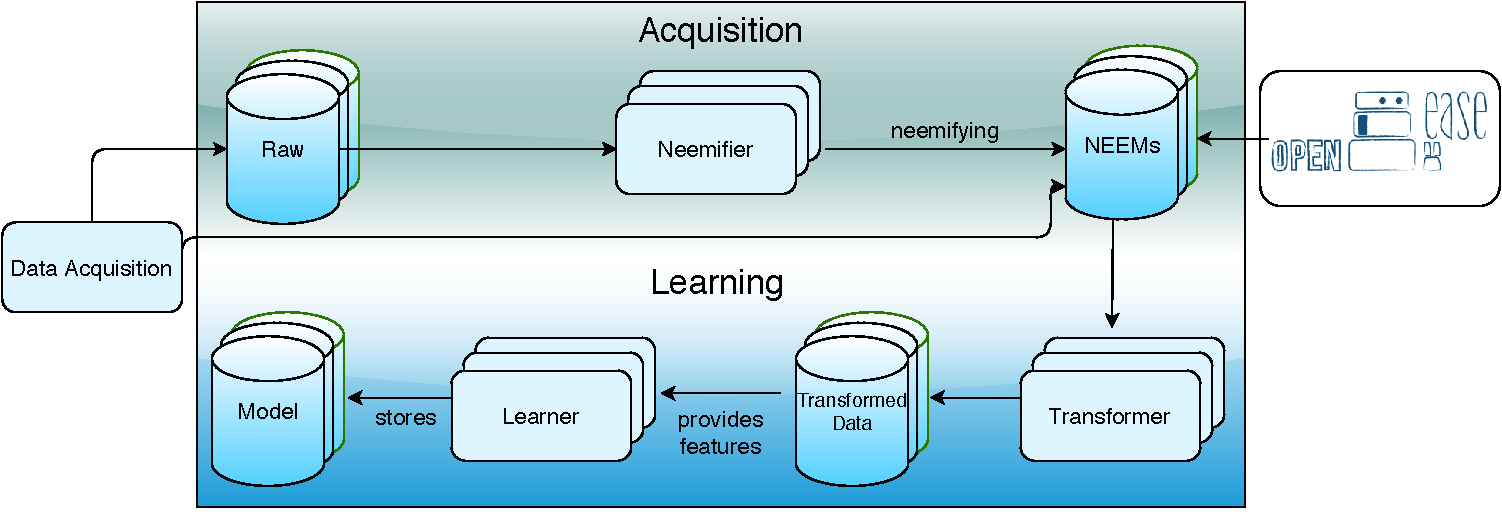
\includegraphics[width=\linewidth]{img/NEEM-Hub.pdf}
	\caption{The NEEM-Hub Architecture}
	\label{fig:neem-hub}
\end{figure} 


Currently, we are only supporting data upload and hosting, like raw data, \neems and transformed data.
In future, we will provide the feature to share your neemifier and transformers with the community and create your own pipelines directly on the \neemhub.
In the rest of this section we will describe how you can upload the data to the \neemhub.

\section{Prerequisite}
\begin{enumerate}
	\item Due to security reasons our Hadoop cluster can be only accessed via the university's intranet right now.	
	\item To be able to publish your data, you are required to have a git account on our GitLab system
	\url{https://neemgit.informatik.uni-bremen.de} 
	\item To support version control with our \neems we have to install DVC \url{https://dvc.org/}, if possible use a precompiled package \url{https://github.com/iterative/dvc.org/blob/master}.
	\item Get familiar with DVC \url{https://dvc.org/doc/start}.
	\item Install Hadoop or a client which can interact with our HDFS filesystem. To install Hadoop on Ubuntu 18.04 you can follow these steps:
	\begin{enumerate}
		\item Install Java 8 if it is not already installed:
\begin{lstlisting}[language=bash, caption=Install Java]
add-apt-repository ppa:webupd8team/java
apt update
apt install -y oracle-java8-set-default
\end{lstlisting}
		\item Download the Hadoop Binaries, untar the archive and move it to /usr/local
\begin{lstlisting}[language=bash, caption=Install Hadoop Binaries]
wget http://apache.claz.org/hadoop/common/hadoop-3.3.1/hadoop-3.3.1.tar.gz
tar -xzvf hadoop-3.3.1.tar.gz
mv hadoop-3.3.1 /usr/local/hadoop
\end{lstlisting}
		\item Set the following environment variables so that DVC can find the Hadoop binaries:
\begin{lstlisting}[language=bash, caption=Export environment variables for Hadoop]
export PATH="/usr/local/hadoop/lib/native:/usr/local/hadoop/bin:/usr/local/hadoop/sbin:$PATH"
export ARROW_LIBHDFS_DIR="/usr/local/hadoop/lib/native"
export CLASSPATH=`/usr/local/hadoop/bin/hdfs classpath --glob`
\end{lstlisting}		
	\end{enumerate}
\end{enumerate}

\section{Downloading}

To test if you setup your system successful, you can try to download \neems: 

\begin{enumerate}
	\item You can explore a DVC repository using \emph{dvc list}:
\begin{lstlisting}[language=bash, caption=Exploring a DVC repository using \emph{dvc list}]
dvc list https://neemgit.informatik.uni-bremen.de/neems/ease-2020-pr2-setting-up-table
\end{lstlisting}
	\item To download specific episodes you can download them using \emph{dvc get}:
\begin{lstlisting}[language=bash, caption=Downloading a episode using \emph{dvc get}]
dvc get https://neemgit.informatik.uni-bremen.de/neems/ease-2020-pr2-setting-up-table episodes/1599727087.4392.zip
\end{lstlisting}
	\item To download a complete \neem you can download it by first cloning the repository using \emph{git} and then using \emph{dvc pull}:
\begin{lstlisting}[language=bash, caption=Downloading a \neem using \emph{dvc pull}]
git clone https://neemgit.informatik.uni-bremen.de/neems/ease-2020-pr2-setting-up-table
cd ease-2020-pr2-setting-up-table
dvc pull
\end{lstlisting}
\end{enumerate}

\section{Publishing}
To organized the raw and transformed data and the \neems, we created 3 groups on GitLab.
Each group corresponds to the specific data set type.
The general procedure to publish your data set is that you create a git repository in the corresponding group. The following is an example step by step guide on how to publish a dataset, in this case a NEEM:

\begin{enumerate}
	\item Create a repository in the \neem group \url{https://neemgit.informatik.uni-bremen.de/neems}
	\item Clone the empty repository and initialize DVC in this repository
\begin{lstlisting}[language=bash, caption=Initialize DVC using \emph{dvc init}]
git clone git@neemgit.informatik.uni-bremen.de:neems/hello-neem2.git
cd hello-neem2
dvc init
\end{lstlisting}
	\item Define the remote storage, to let DVC store your data set:
\begin{lstlisting}[language=bash, caption=Define remote storage using \emph{dvc remote add}]
dvc remote add -d origin hdfs://hadoop@134.102.137.65:9000/neems/hello-neem2
\end{lstlisting}	
\item You can now add your episodes via DVC and push it:
\begin{lstlisting}[language=bash, caption=Add data and pushing using \emph{dvc add} and \emph{dvc push}]
dvc add episodes/1599727087.4392.zip
dvc push
\end{lstlisting}
\item After pushing your data, you still need to push the DVC data placeholder\footnote{.dvc files: https://dvc.org/doc/user-guide/project-structure/dvc-files}:
\begin{lstlisting}[language=bash, caption=Downloading a \neem using \emph{dvc pull}]
git add episodes/1599727087.4392.zip.dvc
git commit -m "Some commit message"
git push
\end{lstlisting}
\end{enumerate}

Publishing other data set types will work in a familiar fahion, but you need to create the repository in the corresponding group and define the remote storage based on your data set type:
 
\begin{description}
	\item[\textbf{Raw data}]\leavevmode \newline
		\url{hdfs://hadoop@134.102.137.65:9000/raw/<your-repo-name>}
	\item[\textbf{\neems}] \leavevmode \newline
		\url{hdfs://hadoop@134.102.137.65:9000/neems/<your-repo-name>}
	\item[\textbf{Transformed Data}] \leavevmode \newline
		\url{hdfs://hadoop@134.102.137.65:9000/transformed_data/<your-repo-name>}
\end{description}

In future, you will be able to publish your neemifier and transformers.
This will allow to share your tools easily with the community and also automatize your data transformation and learning pipeline.




\setcounter{section}{0}
\chapter{NEEM-Acquisition}
\label{ch:acquisition}
\chapterauthor{S. Koralewski, A. Hawkin}

This chapter focuses on the acquisition process of \neems.
At first, we will provide the tools and procedures to acquire episodic memories from robots performing experiments.
The second section focuses on the \neem acquisition from virtual reality. 

%Each section will contain an example \neem to provide insights on, how the representation, described in the chapters \ref{ch:background}, \ref{ch:narrative} and \ref{ch:experience} is utilized to capture performed activities by robots or by humans. 
%In addition, each example \neem is available on the \neemhub for downloading.



\section{Data Structure}

We are using MongoDB to capture the data structures of the \neems.
If you will use the \knowrob interface to create your \neems then your \neem will consist of at least 3 folders - \textit{annotations}, \textit{inferred} and \textit{triples}.
The \neemnar and \neemexp are stored as a collection of BSON \footnote{http://bsonspec.org/faq.html} files.
Each folder should contain a BSON file and metafile stored as JSON. The metafile will include additional information related to \neems. This additional meta information is useful for searching \neem on \openease platform and hence needs to be provided by \neem creator while \neem acquisition time. An example of such information is as displayed below:

\begin{lstlisting}[language=json,firstnumber=1]
{
	"_id" : ObjectId("5f22b1f512db5aed7cd1961b"), 
	"created_by" : "seba",
	"created_at" : "2020-07-21T06:54:25+00:00",
	"model_version" : "0.1",
	"description" : "NEEM for robot making pizza.",
	"keywords" : [	
	"Pizza",
	"Robot"
	],
	"url" : "Placeholder for the NEEM hub repository url",
	"name" : "NEEM for robot making pizza",
	"activity" : {
		"name" : "Pizza making",
		"url" : "Placeholder for the url/uri of Activity concept defined in ontology"    
	},
	"environment" : "Kitchen",
	"image" : "placeholder for image url for showing neem image on openEASE",  
	"agent" : "Robot"
}
	
\end{lstlisting}

Each generated \neem stores also the complete state of the \soma ontology which was used during the acquisition process.
The benefit of this is that while loading a \neem, it is not required to keep track to load the correct \soma version.
In the following, we will give an overview which information is contained in those folders generated by \knowrob:


\begin{description}
	\item[\textbf{annotations}] The annotations collection contains annotations(comments) which are asserted to the concepts of the ontology.
	\item[\textbf{inferred}] The inferred collection contains triples which were inferred and not asserted during the logging process. Inference processes can be triggered when triples are asserted directly to the knowledge base.
	\item[\textbf{triples}] The triples collection contains all triples which were asserted into the knowledge base during run time.
\end{description}

\subsection{Triple data as JSON object}
	Triple data can also be provided in form of JSON documents, where triples are represented as subject, predicate and object. Subjects and objects are identified by an Internationalized Resource Identifier (IRI), which is pointing to concepts or instances defined in the \soma ontology. A triple can either link subject with an object, or can link subject with data value which is represented using one of the base types: string, boolean, and a number. Whereas, the predicate is named by the IRI pointing to property concepts mentioned in the \soma ontology. It is also possible to provide additional time scope fields `since` and `until` to indicate that the given triple is valid for the given time scope. These values are considered here in seconds from when an experiment has started being recorded. An example of such a JSON document is given below where the \emph{Salad\_PMRVYPJH} has a \emph{patient} role from 27.739th second till 29.075. By default triple is valid for the infinite time when the scope parameters are not specified. 
\begin{lstlisting}[language=json,firstnumber=1]
[
 {
   "s": "http://www.ease-crc.org/ont/SOMA.owl#Salad_PMRVYPJH",
   "p": "http://www.ontologydesignpatterns.org/ont/dul/DUL.owl#hasRole",
   "o": "http://www.ease-crc.org/ont/SOMA.owl#Patient_YGJUVNDR",
   "since": 27.739,
   "until": 29.075
 }
]
\end{lstlisting}

It is important to note that, this is an intermediate data format which is not equivalent with how the NEEM narrative is actually stored in databases.
The format described here rather serves as an easy-to-use interchange format.

\input{content/acquisition/robot-neem/robot-neem}
\input{content/acquisition/vr-neem/vr-neem}



\setcounter{section}{0}
\chapter{NEEM Quick-start Guide}
\label{ch:initial_checklist}

In this chapter we give a checklist for the \neems creation process to help the users in generating \neems in case no existing NEEM-logger can be used. 

\section{NEEM Checklist}

\subsection{Necessary files}
\label{sec:checklist_files}

You should have the following files available:

\begin{itemize}
	\item Agent meshes and urdf files are available
	\item Agent owl file corresponding to urdf needs to be created
	\begin{itemize}
		\item Required kinematic information is provided in owl file pointing to correct urdf file name 
	\end{itemize}
	\item Environment meshes and urdf files are available
	\item Environment owl file corresponding to urdf needs to be created
	\begin{itemize}
		\item Required kinematic information is provided in owl file pointing to correct urdf file name
	\end{itemize}
\end{itemize}

\subsection{Data formats}

The data should automatically be in the correct format if KnowRob is used to log the tf and triple information. If the data was recorded without using Knowrob, please follow the checklist below:

\begin{itemize}
	\item Make sure if tf data is available in correct format
	\begin{itemize}
		\item Tf data is provided as individual json documents not as the list/array of json documents.
		\item The coordinate system is right handed
		\item Correct tf tree is presented in the data
		\item Joint rotation is provided in quaternion
		\item Position data is logged in meters
	\end{itemize}
	\item Make sure if triple data is available in correct format
	\begin{itemize}
		\item Triple data is provided as an array of json document
		\item Correct \soma concepts used from \neemnar part
	\end{itemize}
\end{itemize}

\subsection{Semantic Annotation}
\label{sec:semantic_annotation}

In this chapter we discuss the necessary semantic annotation that is stored in the triple collection. First we will list the semantic information that is necessary to generate a simple NEEM:

\begin{itemize}
	\item Necessary steps when starting the logging:
	\begin{itemize}
		\item Create the episode and add dul:isSettingFor relation between the episode and the robots and locations (see \ref{sec:episodes})
	\end{itemize}
	\item Create an hierachy of actions
	\begin{itemize}
		\item Add the task that is executed during the action (see \ref{sec:classification})
		\item Add start and endtime (as unix timestamps) to action (see \ref{sec:occurrences})
		\item Repeat the above points for all sub-actions of the Action-Hierachy, and link them to the parent-actions (see \ref{sec:composition})
		\item For the top-level action: Link the action to the created Episode
	\end{itemize}
\end{itemize}

Now we we will list some additional semantic annotation that would be helpful for the future use of the logged NEEM:

\begin{itemize}
	\item Add additional informations to better classify an action: 
	\begin{itemize}
		\item Add the performing agents (see \ref{sec:participation})
		\item Add objects that are participating in the action (see \ref{sec:participation})
		\item Add conceptualization to the objects in an action by adding roles (see \ref{sec:narrative:roles})
		\item Add executed motions to an action (see \ref{sec:narrative:events})
	\end{itemize}
\end{itemize}

In general, additional semantic annotations can be added as needed. In the next chapter we show how this annotation can be implemented with KnowRob.

\subsection{Semantic Annotation: KnowRob}
\label{sec:semantic_annotation_knowrob}

The easiest way to generate a correct semantic annotation described in \ref{sec:semantic_annotation} is using KnowRob. First we will describe which queries are necessary to generate a simple NEEM. The used concepts for agents, objects, roles etc. are examples. Please find the correct concepts for your usage in SOMA\footnote{https://ease-crc.github.io/soma}.

\begin{itemize}
	\item Necessary steps when starting the logging:
	\begin{itemize}
		\item Load the OWL Files collected according to \ref{sec:checklist_files}, e.g.: 
			\begin{lstlisting}[language=Prolog]
tripledb_load('package://knowrob/owl/robots/PR2.owl')
			\end{lstlisting}
		\item Load the URDF Files and link them to the corresponding robot/location from the OWL File, e.g.:
		\begin{lstlisting}[language=Prolog]
urdf_load('http://knowrob.org/kb/PR2.owl#PR2_0', 'package://knowrob/urdf/pr2.urdf', [load_rdf])
		\end{lstlisting}
		\item Create the episode: tell(is\_episode(Episode))
		\item Add setting\_for relations for robots and locations: 
		\begin{lstlisting}[language=Prolog]
is_setting_for(Episode,'http://knowrob.org/kb/PR2.owl#PR2_0')
		\end{lstlisting}
	\end{itemize}
	\item Log the Action-Hierachy
	\begin{itemize}
		\item Create an action, e.g.:
			\begin{lstlisting}[language=Prolog]
tell(is_action(Action))
			\end{lstlisting}
		\item Add the task that is executed during the action, e.g.: 
			\begin{lstlisting}[language=Prolog]
tell([has_type(Tsk,soma:'Transporting'),
executes_task(Action,Tsk)])
			\end{lstlisting}
		\item Add start and endtime (as unix timestamps) to action, e.g.: 
			\begin{lstlisting}[language=Prolog]
tell(occur(Act) during [Start, End])
			\end{lstlisting}
		\item Repeat the above points for all sub-actions of the Action-Hierachy, and link them to the parent-actions:
			\begin{lstlisting}[language=Prolog]
tell(has_subevent(ParentAct,Action))
			\end{lstlisting}
		\item For the top-level action: Link the action to the created Episode, e.g.: 
			\begin{lstlisting}[language=Prolog]
tell(is_setting_for(Episode,Action))
			\end{lstlisting}
	\end{itemize}
\end{itemize}

Now we we will list some additional semantic annotation to add more information to the logged NEEM:

\begin{itemize}
	\item Add additional informations to better classify an action: 
	\begin{itemize}
		\item Add the performing agents, e.g.:
			\begin{lstlisting}[language=Prolog]
tell(is_performed_by(Action,pr2:'PR2_0'))
			\end{lstlisting}
		\item Add objects that are participating in the action, e.g.:
			\begin{lstlisting}[language=Prolog]
tell(has_participant(Action,soma:'Milk_0'), \)
			\end{lstlisting}
		\item Conceptualize objects and agents in an action by adding roles, e.g.:
			\begin{lstlisting}[language=Prolog]
tell([has_type(RobotRole, soma:'AgentRole'),' 
		has_role(pr2:'PR2_0', RobotRole) during Action,'])
			\end{lstlisting}
		\item Add executed motions to an action, e.g.:
			\begin{lstlisting}[language=Prolog]
tell([has_type(Mot,soma:'LimbMotion'),
       is_classified_by(Action,Mot)])
			\end{lstlisting}
	\end{itemize}
\end{itemize}

%\subsection{Checks}
%
%\todo{Should this points stay, or do we hope for automatic neem validation in the neemhub?}
%
%You can try the following checks to test if your logged data is correct:
%
%\begin{itemize}
%	\item Validate triple data with \neem validation script??
%	\item Test current neem experiment data (tf, triple, meshes and urdfs) locally with \knowrob, \todo{here not everyone will use knowrob, so some way we need to provide an interface}
% 	\item Agent and environment meshes with urdf files are rendered properly with \knowrob in rviz 
%\end{itemize}

%\input{content/application/application}
%\input{content/future-work/future-work}

\setcounter{section}{0}
\chapter{Appendix}
\label{app:complete_pub_list}


\section{Agent owl file}
\label{appendix:section1}
 

 \definecolor{codegreen}{rgb}{0,0.6,0}
 \definecolor{codegray}{rgb}{0.5,0.5,0.5}
 \definecolor{codepurple}{rgb}{0.58,0,0.82}
 \definecolor{backcolour}{rgb}{0.95,0.95,0.92}
 
 \lstdefinestyle{mystyle}{
 	backgroundcolor=\color{backcolour},   
 	commentstyle=\color{codegreen},
 	keywordstyle=\color{magenta},
 	numberstyle=\tiny\color{codegray},
 	stringstyle=\color{codepurple},
 	basicstyle=\ttfamily\footnotesize,
 	breakatwhitespace=false,         
 	breaklines=true,                 
 	captionpos=b,                    
 	keepspaces=true,                 
 	numbers=left,                    
 	numbersep=5pt,                  
 	showspaces=false,                
 	showstringspaces=false,
 	showtabs=false,                  
 	tabsize=2,
 	caption=Agent owl file,
 	label=fig:agent_owl_file
 }
 
 \lstset{style=mystyle}
  
\lstinputlisting[language=XML]{content/appendix/ElanHumanSkeleton.owl}

\section{Environment owl file}
\label{appendix:section2}
 
 

\definecolor{codegreen}{rgb}{0,0.6,0}
\definecolor{codegray}{rgb}{0.5,0.5,0.5}
\definecolor{codepurple}{rgb}{0.58,0,0.82}
\definecolor{backcolour}{rgb}{0.95,0.95,0.92}

\lstdefinestyle{mystyle}{
	backgroundcolor=\color{backcolour},   
	commentstyle=\color{codegreen},
	keywordstyle=\color{magenta},
	numberstyle=\tiny\color{codegray},
	stringstyle=\color{codepurple},
	basicstyle=\ttfamily\footnotesize,
	breakatwhitespace=false,         
	breaklines=true,                 
	captionpos=b,                    
	keepspaces=true,                 
	numbers=left,                    
	numbersep=5pt,                  
	showspaces=false,                
	showstringspaces=false,
	showtabs=false,                  
	tabsize=2,
	caption=Environment owl file,
	label=fig:environment_owl_file
}

\lstset{style=mystyle}

\lstinputlisting[language=XML]{content/appendix/ElanMap.owl}

 

\cleardoublepage
\bibliography{neem}
\bibliographystyle{plain}

%\setcounter{section}{0}
%\chapter{Appendix}
\label{app:complete_pub_list}


\section{Agent owl file}
\label{appendix:section1}
 

 \definecolor{codegreen}{rgb}{0,0.6,0}
 \definecolor{codegray}{rgb}{0.5,0.5,0.5}
 \definecolor{codepurple}{rgb}{0.58,0,0.82}
 \definecolor{backcolour}{rgb}{0.95,0.95,0.92}
 
 \lstdefinestyle{mystyle}{
 	backgroundcolor=\color{backcolour},   
 	commentstyle=\color{codegreen},
 	keywordstyle=\color{magenta},
 	numberstyle=\tiny\color{codegray},
 	stringstyle=\color{codepurple},
 	basicstyle=\ttfamily\footnotesize,
 	breakatwhitespace=false,         
 	breaklines=true,                 
 	captionpos=b,                    
 	keepspaces=true,                 
 	numbers=left,                    
 	numbersep=5pt,                  
 	showspaces=false,                
 	showstringspaces=false,
 	showtabs=false,                  
 	tabsize=2,
 	caption=Agent owl file,
 	label=fig:agent_owl_file
 }
 
 \lstset{style=mystyle}
  
\lstinputlisting[language=XML]{content/appendix/ElanHumanSkeleton.owl}

\section{Environment owl file}
\label{appendix:section2}
 
 

\definecolor{codegreen}{rgb}{0,0.6,0}
\definecolor{codegray}{rgb}{0.5,0.5,0.5}
\definecolor{codepurple}{rgb}{0.58,0,0.82}
\definecolor{backcolour}{rgb}{0.95,0.95,0.92}

\lstdefinestyle{mystyle}{
	backgroundcolor=\color{backcolour},   
	commentstyle=\color{codegreen},
	keywordstyle=\color{magenta},
	numberstyle=\tiny\color{codegray},
	stringstyle=\color{codepurple},
	basicstyle=\ttfamily\footnotesize,
	breakatwhitespace=false,         
	breaklines=true,                 
	captionpos=b,                    
	keepspaces=true,                 
	numbers=left,                    
	numbersep=5pt,                  
	showspaces=false,                
	showstringspaces=false,
	showtabs=false,                  
	tabsize=2,
	caption=Environment owl file,
	label=fig:environment_owl_file
}

\lstset{style=mystyle}

\lstinputlisting[language=XML]{content/appendix/ElanMap.owl}

 
\end{document}
